
\newpage
\null\vfill

\begin{figure}
\vspace*{-0cm}
\centering
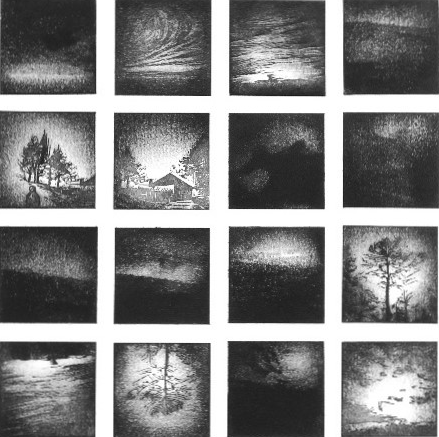
\includegraphics[width = 9cm]{img/cecile_rescan.png}
\caption*{\footnotesize\emph{Linocuts made by Cécile Rescan.}}
\vspace*{-0cm}
\label{fig:gravurececile}
\end{figure}

\vfill\null

\newpage

\subsection*{Remerciements}

{
\small

La réalisation de cette thèse n’aurait jamais été possible sans le soutien de nombreuses personnes que je souhaite remercier ici.

Tout d'abord, un grand merci à Isabelle pour la confiance qu'elle m'a accordée. Nous étions surtout deux dans cette aventure. Malgré tes nombreux engagements académiques, tu as toujours veillé à m'encadrer avec soin et humanité -- et toujours avec une pointe d'humour. Je t'en suis très reconnaissant. Ton dynamisme et ta rigueur scientifique font de toi un vrai modèle de chercheuse. 

Il me semble également important de souligner que ces trois années de thèse ne sont que l'aboutissement de toutes les enseignements de qualité que j'ai eu la chance de recevoir à l'école publique.
Merci donc à tous les enseignants qui ont participé à ma formation -- scientifique ou non-scientifique -- et qui ont su développer ma curiosité intellectuelle depuis mon enfance jusqu'à l'Agro.

Je souhaite également remercier Bruno Hérault et Emmanuelle Porcher, qui m'ont tous les deux accueilli pour des stages il y a quelques années. Votre encadrement stimulant et bienveillant est en grande partie responsables de mon goût pour la recherche. Vous m'avez offert l'opportunité de travailler sur des sujets passionnants, et m'avez fait confiance pour mener des projets scientifiques jusqu'au bout.
Vous m'avez donné l'envie de faire une thèse, et je suis aussi certain que c'est un peu grâce à vous que j'ai pu obtenir le financement de ce travail.

Un grand merci à toute l'équipe Forecast pour avoir su constamment maintenir une ambiance décontractée dans le couloir. Merci à Florent (ne change rien !), Jean, Damien, les deux Jean-Marc, Xavier, Florence, et toutes celles et ceux que j'ai croisés de près ou de loin. Bien évidemment, merci à Lilian (\emph{from Morteau University}) de m'avoir supporté tout au long de ces 3 ans. Merci aussi à Marie-Charlotte, tu es une amie précieuse.\\
Je souhaite aussi remercier tous les collègues qui m'ont accompagné dans ce travail et l'ont enrichi, et notamment Frédérik Saltré et Hendrik Davi. 

J'en profite également pour remercier Lizzie Wolkovich. Tu as toujours été à l'écoute lors de tes séjours en France et tu as toujours accepté avec bonne humeur de donner ton avis sur ce travail. Et surtout, merci pour l'opportunité de continuer la recherche à tes côtés à Vancouver dès l'année prochaine~: \emph{I can't wait!}

Je souhaite remercier sincèrement la rapportrice et le rapporteur, Marta Benito-Garzón et Jérome Chave, ainsi que les examinatrices et les examinateurs, Isabelle Boulangeat, Christophe Botellat et Rachid Cheddadi, pour l’honneur qu’ils me font de participer à mon jury de thèse. Merci d'avoir accepté de prendre le temps d'évaluer ce travail, je vous en suis très reconnaissant. \\
Merci aussi aux membres de mon comité de thèse qui m'ont suivi pendant ces 3 ans et m'ont donné de précieux conseils : Christelle Hély-Alleaume, Marie Launay, Nicolas Viovy, Vincent Devictor et Olivier Gimenez.

J’aimerais clôre ces remerciements par ma famille, mes amis, et en particulier Ombeline.
J'ai hâte de continuer ce chemin à tes côtés.
}

\freefootnote{\scriptsize Merci également à \href{https://github.com/sylvainschmitt}{Sylvain Schmitt} dont j'ai réutilisé le template Latex pour écrire ce manuscrit.}